
\section{Basic Definitions}

\subsection{Stochastic Processes}

A \emph{stochastic process} $p$ is a $\mathcal{T}$-indexed family of
random variables $X_i$, formally $p = \{X_i: i \in \mathcal{T}\}$, in
particular $p$ is called \emph{discrete} if $\mathcal{T} = \mathbb{N}
$, otherwise $p$ is called \emph{continuous} if $\mathcal{T} =
\mathbb{R} $.


\subsection{Discrete Time Markov Chains}

A \emph{Discrete Time Markov Chain} (DTMC) is a discrete stochastic
process such that, given $\Omega$ a sample space, $X_i:\Omega
\rightarrow \mathbb{N}, \forall i\in \mathbb{N} $.

\subsection{Continuous Time Markov Chains}

A \emph{Continuous Time Markov Chain} (CTMC) is a continuous
stochastic process such that, given $\Omega$ a sample space,
$X_i:\Omega \rightarrow \mathbb{R}, \forall i\in \mathbb{R} $.


% Usually a DTMC is
% modeled with a tuple $(S, P, AP, L)$ such that:
% \begin{itemize}
% \item $S$ is a finite set of \emph{states};
% \item $P$ is a function such that $P:S\times S \rightarrow [0,1]$,
%   where $\sum_{v \in S}{P(s,v)} = 1, \forall s \in S $;
% \item $AP$ is a set of \emph{atomic propositions};
% \item $L$ is a function such that $L:S \rightarrow AP$.
% \end{itemize}

\section{Herman's Stabilization algorithm}

This paper study an algorithm about self-stabilization of
fault-tolerant systems in a distributed environment. We can abstract a
fault-tolerant system with a network of processes and the goal is to
build a protocol which, applied to an initial configuration $i$ of the
network, produces a new configuration $c$ such that:
\begin{itemize}
\item $c$ satisfies some property of interest;
\item the protocol requires a \emph{finite} number of steps to produce
  $c$;
\item there is no intervention of outside objects in order to produce
  $c$.
\end{itemize}
In the following section we state formally the problem described above
and the Herman algorithm under study. We've used the article \cite{
  KNP12a} to make our abstractions.

\subsection{Model}

Herman protocol \cite{Her90} is applied to a network of processes
$p_i$ where $i \in \{1,\ldots, n\}$, structured in an oriented ring
and ordered anticlockwise. This protocol is synchronous, that is
actions taken by each process $p_i$ happen simultaneously, no
interleaving are present. Following the presentation given by Herman,
it is possible to represent each process $p_i$ with a single
\emph{bit} $x_i$ and the entire network with a DTMC. With those basics
we're ready to introduce some concepts that we want to study with a
simulation using PRISM \cite{KNP11}.

We define a \emph{network configuration} as a state of the DTMC with
$n$ processes, so a tuple $(x_n, \ldots, x_1) \in \{0,1\}^n$. In the
ring may exist one or more processes that have \emph{tokens} and those
can be passed between processes $p_i$ and $p_{i+1}$ (so always to the
right neighbor). A process $p_i$ has a token if $x_i = x_{i-1}$ ($x_1
= x_n$ due to ring network structure). Finally, a network
configuration is \emph{stable} if $\exists! p_i$ that has a token.
\\\\
From the above definitions follow these facts:
\begin{itemize}
\item given a network with $n$ processes, the set of states $S$ of the
  underlying DTMC has $2^n$ states. This can be proved saying
  that each state $s\in S$ has $n$ components, each component has $2$
  possible value, hence $|S| = 2^n$;
\item given a network with $n = 2k+1$ processes, there no exists
  network configuration with $t=2j$ tokens. To see why we use a
  constructive proof:
  \begin{proof} Let $(x_n,x_{n-1}, \ldots, x_2,x_1)$ be a network
    configuration such that $n=2k+1$ and $(x_{n-1}, \ldots,x_2, x_1)$
    be a suffix with $t=2j$ tokens (which is perfectly legal, for
    instance $(0,0,1,1,0,0)$, with tokens in $p_6, p_4, p_2, p_1$).

    Suppose $x_1 = 0$ (the same argument may be applied for
    $x_1=1)$. We can have the following suffixes with even length:
    \begin{itemize}
    \item $(0,x_{n-2},\ldots, x_2,0)$, we can complete it by adding
      $x_n$ such that:
      \begin{itemize}
      \item $(0,0,x_{n-2},\ldots, x_2, 0)$ in this configuration there
        are $2j+1$ token (one more due to $(x_n,x_{n-1})$);
      \item $(1,0,x_{n-2},\ldots, x_2,0)$ in this configuration there
        are $2j-1$ token (one less due to breaking $(x_1,x_{n-1})$);
      \end{itemize}
    \item $(1,x_{n-2},\ldots, x_2,0)$, we can complete it by adding
      $x_n$ such that:
      \begin{itemize}
      \item $(0,1,x_{n-2},\ldots, x_2, 0)$ in this configuration there
        are $2j+1$ token (one more due to $(x_1,x_n)$);
      \item $(1,1,x_{n-2},\ldots, x_2,0)$ in this configuration there
        are $2j+1$ token (one more due to $(x_n,x_{n-1})$).
      \end{itemize}
    \end{itemize}
    Adding $x_n$ on configurations of even length we get $2j\pm 1 $
    tokens, which is an odd number.
  \end{proof}
\end{itemize}

\subsection{Protocol rule}

Let $k$ be a generic execution step, the protocol consists of the
following rule:
\begin{displaymath}
  \begin{split}
    x_{i}^{(k+1)} &:= x_{i-1}^{(k)} \quad &\text{if } x_{i}^{(k)} \not=
    x_{i-1}^{(k)}\\
    x_{i}^{(k+1)} &:= random(0,1) \quad &\text{if } x_{i}^{(k)} =
    x_{i-1}^{(k)}
  \end{split}
\end{displaymath}
where $x_{i}^{(k)}$ is the value of $x_i$ at step $k$, $:=$ means
assignment and $random$ is a function that simulate a unbiased coin
toss. In \autoref{table:herman-protocol-execution-example} we report a
simple example of protocol execution applied to 5 processes, starting
from the network configuration $(1, 1, 0, 0, 1)$.
\begin{table}[ht]
  \begin{center}
    \begin{tabular}{cccc}
      \hline
      step & $(x_5, x_4, x_3, x_2, x_1)$ & Tokens owners & coin tosses \\ 
      \hline     
      1 & $(1, 1, 0, 0, 1)$ & $p_5, p_3, p_1$ & $x_1^{(2)}:= 0,
      x_3^{(2)}:= 1, x_5^{(2)}:= 1$  \\
      2 & $(1, 0, 1, 1, 0)$ & $p_3$ & $x_3^{(3)}:= 0$  \\
      3 & $(0, 1, 0, 0, 1)$ & $p_3$ & $x_3^{(4)}:= 0$  \\
      4 & $(1, 0, 0, 1, 0)$ & $p_4$ & $x_4^{(5)}:= 0$  \\
      5 & $(0, 0, 1, 0, 1)$ & $p_5$ & $\ldots$  \\ 
      \hline
    \end{tabular}
    \caption{Example of protocol execution}
    \label{table:herman-protocol-execution-example}
  \end{center}
\end{table}

It is interesting to observe these facts:
\begin{itemize}
\item from network configurations $\forall i:x_i=0$ and $\forall
  i:x_i=1$ of length $n$, it is possible to reach every other state by
  applying the second case of the protocol rule;
\item the protocol doesn't stop when a stable network configuration is
  reached. In fact, in a stable configuration, let $p_i$ be the token
  owner: depending its coin tossing, $p_i$ can decide to pass the
  token to $p_{i+1}$ or to keep it another turn (in the example
  reported above, if at step 4 would have been $x_4^{(5)}:= 1$ the
  next configuration would have been $(0, 1, 1, 0, 1)$, with $p_4$
  token owner again);
\item in order to have an estimate number of steps necessary to reach
  a stable configuration we do a PRISM simulation, using the
  \emph{Confidence Interval} method, with 1000 samples. Looking at the
  log:
\begin{verbatim}
Path length statistics: average 5.4, min 1, max 29
\end{verbatim}
  So the average number of necessary steps for reaching a stable
  configuration is $5.4$.
\end{itemize}

\subsection{Interesting properties}

In this section we verify if Herman protocol satisfy some desired
properties, in particular if a stable configuration is eventually
reached and if it is reached within $k$ steps.

Before get deep into properties verification it is important to
understand that if we'd have used a \emph{qualitative} model checker
to verify if a stable configuration is \emph{always} eventually
reached, the result would be \emph{reject}. To see why, let the DTMC
be in the state $(1,1,1,1,\ldots,1,1)$ and, repeating the application
of rule two of the protocol, for all $p_i$ the coin toss results in
$1$, getting $(1,1,1,1,\ldots,1,1)$ again. There exists an infinite
path on the DTMC which catch the previous behavior, hence that path is
the counterexample for ``from the initial state
$(1,1,1,1,\ldots,1,1)$, is a stable configuration \emph{always}
eventually reached?''

\subsubsection{One initial state $(1,1,1,\ldots,1,1)$}

In \autoref{table:herman-initial-states-properties-results} we report
the properties that we've verified with PRISM, the label ``stable''
represent a predicate such that:
\begin{displaymath}
  \begin{split}
    \text{stable is true} \leftrightarrow 1 = &(x_1=x_2?1:0)+(x_2=x_3?1:0)+(x_3=x_4?1:0)+(x_4=x_5?1:0)\\
    &+(x_5=x_6?1:0)+(x_6=x_7?1:0)+(x_7=x_1?1:0)
  \end{split}
\end{displaymath}


\begin{table}[ht]
  \begin{center}
    \begin{tabular}{p{5cm}cc}
      \hline
      description & PRISM property  & result \\
      \hline     
      from the initial state, a stable state is reached with
      probability 1 & P>=1 [ F "stable" ] & true \\
      from the initial state, a stable state is reached within 10
      steps with probability 1 & P>=1 [ F<=10 "stable" ] & false\\
      from the initial state, a stable state is reached within 10
      steps with probability .5 & P>=.5 [ F<=10 "stable" ] & true\\
      from the initial state, what is the probability to reach a
      stable state within 10 steps? & P=? [ F<=10 "stable" ] & .8757\\
      what is the expected number of steps required for the
      self-stabilization algorithm to reach a stable state? & R=? [ F
      "stable" ] & 5.4933\\
      \hline
    \end{tabular}
    \caption{Properties and their verification using a single initial
      state}
    \label{table:herman-initial-states-properties-results}
  \end{center}
\end{table}

\subsubsection{Multiple initial states}

In \autoref{table:herman-log-chunck-multi-initial-states} we report
the verification of the following property, which informally states:
``what is the maximum/minimum expected time to reach a stable state,
starting from any initial configuration in which there are k tokens?''
\begin{displaymath}
  filter(m, R=? [ F "stable" ], "k\_tokens") \quad m \in \{max, min\}
\end{displaymath}
that we've verified with PRISM considering all states of the DTMC as
an initial state. The label ``stable'' is the predicate defined in the
previous section and ``k\_tokens'' represent a predicate $tokens(k)$
such that:
\begin{displaymath}
  \begin{split}
    tokens(k) \text{ is true } \leftrightarrow k = &(x_1=x_2?1:0)+(x_2=x_3?1:0)+(x_3=x_4?1:0)+(x_4=x_5?1:0)\\
    &+(x_5=x_6?1:0)+(x_6=x_7?1:0)+(x_7=x_1?1:0)
  \end{split}
\end{displaymath}

\begin{table}[ht]
  \begin{center}
    \begin{tabular}{cccc}
      \hline
      tokens & sat states (out of 128)  & maximum over filter &
      minimum over filter \\ 
      \hline     
      1 & 14 & 0 & 0 \\
      3 & 70 & 6.857 & 2.857  \\
      5 & 42 & 5.973 & 5.018  \\
      7 & 2 & 5.493 & 5.493  \\ 
      \hline
    \end{tabular}
    \caption{Property verification about multi initial states}
    \label{table:herman-log-chunck-multi-initial-states}
  \end{center}
\end{table}

In \autoref{fig:herman-plot-output} we report a plot of the results
shown in \autoref{table:herman-log-chunck-multi-initial-states}.
\begin{figure}[htb]
  \centering
  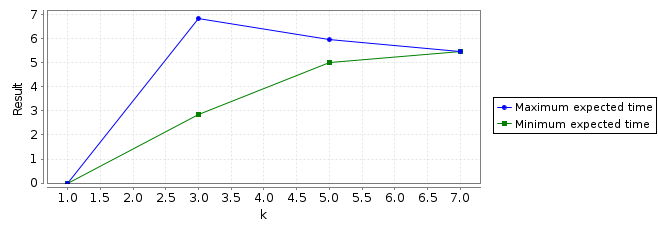
\includegraphics[width=13cm]{quantitative-project/max-min-expected-time-experiment.png}
  \caption{Max/min needed time to reach stable conf against
    tokens quantity}
  \label{fig:herman-plot-output}
\end{figure}

\section{Dynamic power management}

In this section we'll study a \emph{dynamic power management} (DPM)
system, a generalized version of a model presented in \cite{QWP99}
which concerns the model of a 3 state Fujitsu disk drive.

DPMs are interesting to study because they occur every time a device
(or, more generally, a service provider) is present, such that the
device has multiple power states with the following constraints:
\begin{itemize}
\item each state has a different power consumption associated to;
\item each state has a different response time when a service is to be
  performed.
\end{itemize}
The analysis of those model has the goal to reach a reasonable
trade off between the power consumption and the delivered level of
service, that is, having power consumption as low as possible and
quality of service as high as possible.
\\\\
In the following sections we'll build three implementations, each of
them with little differences respect the others, leaving some freedom
degrees which allow us to understand how changes impact on power
consumption and quality of service.

\subsection{First model: Service Queue and Service Provider}

The first model we've implement is composed by the following
components:
\begin{itemize}
\item a \emph{Service Queue} which registers generic service
  requests. We fix an upper bound $q_{max} = 20$ for its size and
  build a PRISM module with $0,\ldots,q_{max}$ states, each of them
  represent the number of service requests asked up to a time $t$. The
  initial state of the \emph{Service Queue} is $0$, an empty queue,
  and a new request arrive every $.72$ seconds.
\item a \emph{Service Provider} which carry out requests. This
  component has three states: \emph{sleep, idle, busy}, with
  \emph{idle} is the initial state. We build a PRISM module with a
  variable such that it ranges over $\{0,1,2\}$ to cover the states of
  the component. The service provider serve a request every $.008$
  seconds. The Service Provider makes a transition from \emph{idle} to
  \emph{busy} whenever a request arrives, while it makes a transition
  from \emph{busy} to \emph{idle} whenever it finishes the service of
  the last request.
\end{itemize}
This two components cannot take actions independently, they must
synchronize for:
\begin{itemize}
\item receiving a request (in order to enque it correctly and moving
  the provider in a \emph{busy} state because there's some work to get
  done);
\item serving a request: this can result in a non empty queue if, in
  the previous state there are at least 2 requests in queue, therefore
  the provider has work to done again; or it can result in an empty
  queue if, in the previous state there are exactly one request in
  queue, therefore the provider has no request to handle, so it can
  move to \emph{idle} state.
\end{itemize}

\subsubsection{Implications}

From the modules' definitions reported above follow this facts:
\begin{itemize}
\item the total number of states of the PRISM system is
  $|\{0,\ldots,q_{max}\} \times \{0,1,2\}| = 63$ as confirmed by the
  log, looking for the dimension of the rate matrix;
\item from the initial state, that is when the queue is \emph{empty}
  and the Service Provider is \emph{idle}, it is possible to reach
  only one state due to the synchronization on action \emph{request}:
  this state record that in the queue there is exactly one element and
  the Service Provider is \emph{busy}.
\end{itemize}

\subsubsection{``Always accept requests and never serve them'' path
  and property on \emph{sleep} state}

It is interesting to report a simple simulation case which study a
``particular'' path of the system, the one in which the system always
choose to accept requests and never serves them. In
\autoref{fig:first-model-saturation-queue} we report this
behavior. The plot is obtained exporting the path and loading the
exported data in a R interpreter to plot the curve: the system, when
the queue is full of requests, rejects every new one.
\begin{figure}[htb]
  \centering
  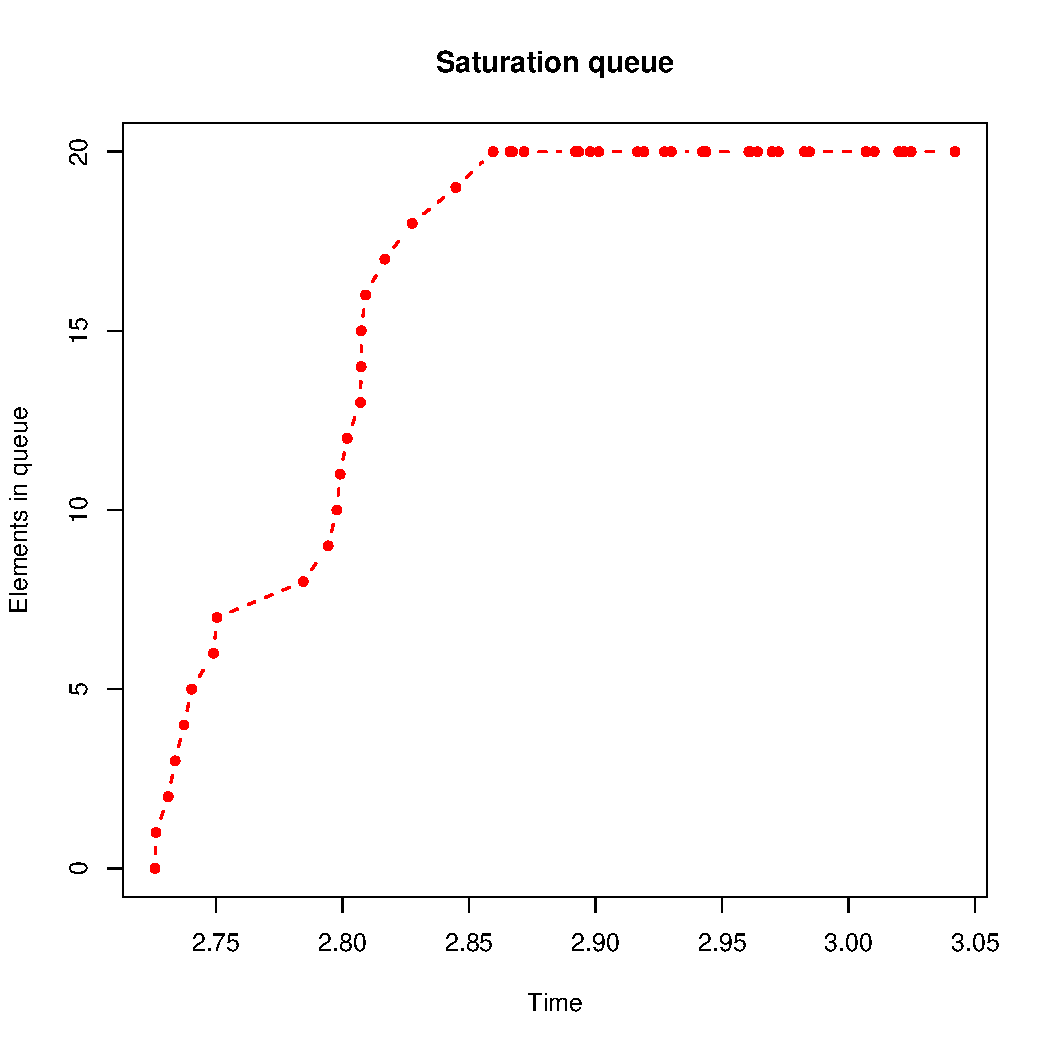
\includegraphics[width=13cm]{quantitative-project/r-project/saturation-queue.pdf}
  \caption{Queue saturation over time if a simulation path always
    choose to accept requests and never serves them}
  \label{fig:first-model-saturation-queue}
\end{figure}

To finish the discussion about this first model we study if it is
possible for the service provider to enter a \emph{sleep} state. In
order to do that we verify the following PRISM property, where $sp=0$
is a true predicate if and only if the service provider is in
\emph{sleep} state:
\begin{displaymath}
  P_{<=0} [ F\quad sp=0 ]
\end{displaymath}
which holds, hence in this PRISM module the service locator never
``\emph{sleep}''.

\subsection{Second model: adding Power Manager}

Look at the previous model: the Service Provider decides for itself
about its state transitions, using a strategy that depends on the
number of requests present in the queue. In this new model we augment
this behavior introducing a new component, a \emph{Power Manager},
which interact with the Service Provider in order to drive its state
transitions, especially between \emph{sleep} and \emph{idle} states.
\\\\
We build a new PRISM model for the Power Manager, which synchronize
the Service Provider to make the following transitions. Let
$q_{trigger}$ be a freedom degree which represent a state of the
queue:
\begin{itemize}
\item $sleep \rightarrow idle$ if the current number $q$ of waiting
  requests in queue is such that $q \geq q_{trigger}$: this transition
  requires $1.6$ seconds;
\item $idle \rightarrow sleep$ if the current number $q$ of waiting
  requests in queue is such that $q = 0$: this transition requires
  $.67$ seconds.
\end{itemize}
With the introduction of the Power Manager we check immediately that
the Service Provider reach a \emph{sleep} state sooner or later. We
verify the following:
\begin{displaymath}
  P_{>=1} [ F\quad sp=0 ]
\end{displaymath}
which holds in this model while in first one doesn't.

In the following paragraphs we'll study some properties of interest
which regard transient and long-run probability of: a full queue,
expected queue size, cumulative missed requests and expected power (for
the latter ones we need to introduce some \emph{rewards structures}).

\subsubsection{Transient and steady-state probability of a full queue}

In \autoref{fig:transient-probability-full-queue} we report a plot of
an experiment concerning the \emph{transient} probability of the queue
being full in order to see if it stabilize after an amount of
time. The experiment stress the following formula:
\begin{displaymath}
  P_{=?} [ F[T,T]\quad q=q_{max} ]
\end{displaymath}
The transient probability stabilizes around .001 as confirmed by the
\emph{green} curve which extends up to time 40, continuing the
\emph{blue} curve which stops at time 20 instead.
\begin{figure}[htb]
  \centering
  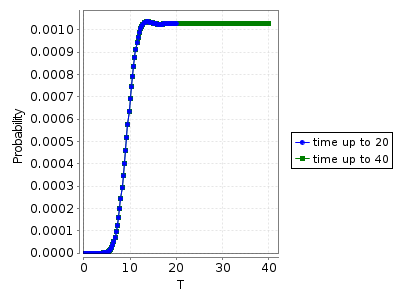
\includegraphics[width=13cm]{quantitative-project/transient-probability-full-queue.png}
  \caption{Transient probability of the queue being full}
  \label{fig:transient-probability-full-queue}
\end{figure}
It is possible to verify the previous result using another property
which uses the \emph{steady states} operator:
\begin{displaymath}
  S_{=?} [ q=q_{max} ]
\end{displaymath}
verifying the property we get .001028, in other words: ``starting from
the initial state, the steady-state (long-run) probability of having a
full queue equals .001028''. We reached this result using the
Gauss-Seidel numerical method because the Jacobi method (the default
one in PRISM) didn't converge in this case.

\subsubsection{Transient and steady-state expected queue size}

In \autoref{fig:expected-queue-size} we report a plot of an experiment
concerning the transient probability of the queue size. To perform the
experiment we need to introduce the following \emph{rewards
  structure}:
\begin{verbatim}
rewards "queue_size"
	true : q;
endrewards
\end{verbatim}
which assigns as ``rewards'' to a state $s$ the number $q$ of requests
present in queue when the system is in state $s$. After we stress the
following formula:
\begin{displaymath}
  R\{"queue\_size"\}_{=?} [ I=T ]
\end{displaymath}
The transient probability stabilizes around 3.2 as confirmed by the
\emph{blue} curve which stops at time 20.
\begin{figure}[htb]
  \centering
  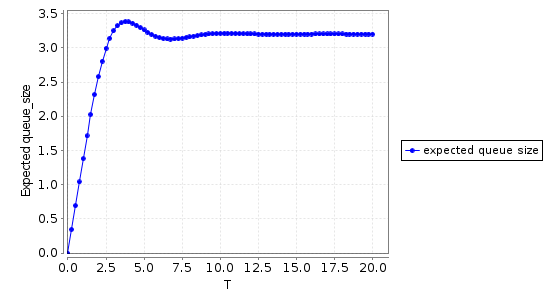
\includegraphics[width=13cm]{quantitative-project/expected-queue-size.png}
  \caption{Expected queue size}
  \label{fig:expected-queue-size}
\end{figure}
It is possible to verify the previous result using another property
which uses the \emph{steady states} operator:
\begin{displaymath}
  R\{"queue\_size"\}_{=?} [ S ]
\end{displaymath}
verifying the property we get 3.20388, in other words: ``starting from
the initial state, in the long-run the expected size of the queue
equals 3.20388''. We reached this result using the Gauss-Seidel
numerical method as did in the previous property.

\subsubsection{Transient expected queue size with multiple values of
  $q_{trigger}$}

The specification of this second model allow us to change
$q_{trigger}$ in order to study how that change impact on the
system. In \autoref{fig:expected-queue-size-multiple-qtrigger} we
report the expected queue size (as done in the previous paragraph)
where $q_{trigger} \in \{4,6,8,10,12,14,16,18\}$.
\begin{figure}[htb]
  \centering
  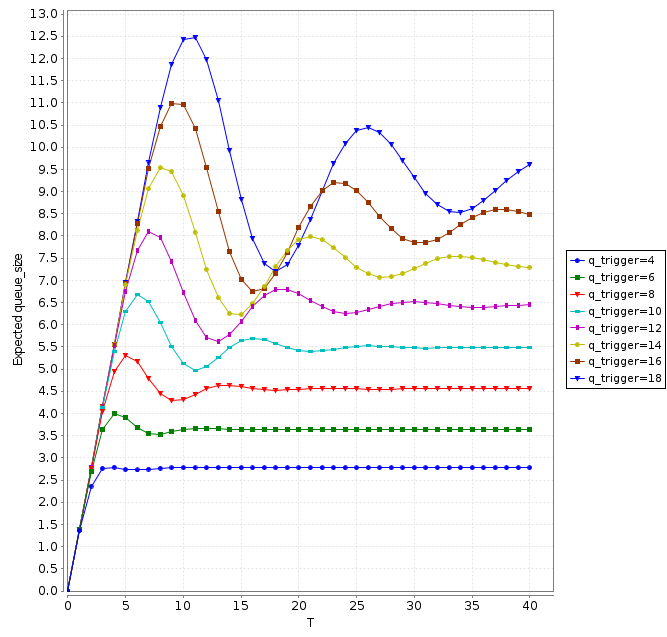
\includegraphics[width=13cm]{quantitative-project/expected-queue-size-multi-q-triggers.png}
  \caption{Expected queue size}
  \label{fig:expected-queue-size-multiple-qtrigger}
\end{figure}
We see that greater $q_{trigger}$ implies more time is needed to
stabilize the queue size. Informally, the more the power manager waits
before synchronizing with the Service Provider, the more
``fluctuations'' the system shows respect to queue size. Of those we
can choose the curve for $q_{trigger}=12$ because it has no common
point with other curves (for instance the blue bigger one for
$q_{trigger}=18$ is better of the curve for $q_{trigger} = 16$ for
$t\in[17, 22]$, but not for $t\in[0,\infty]\setminus[17, 22]$ ) and
takes the queue size under half of the max dimension (in average).

\subsubsection{Transient expected cumulative missed requests }
In this paragraph we study another property about the transient
expected cumulative number of lost requests due to a full queue. As
done in the previous property, we use the same multiple values for
$q_{trigger}$ and we introduce the following rewards structure:
\begin{verbatim}
rewards "lost"
	[request] q=q_max : 1;
endrewards
\end{verbatim}
which assigns a reward of $1$ to a transition $a$ such that:
\begin{itemize}
\item let $p, r \in S$ such that $ p \xrightarrow{a} r$ and $p \vdash
  q= q_{max}$. Informally, the state from which the transition start
  have to be a state where the queue is full;
\item the transition happen due to a synchronization on the action
  \emph{request}. The constraint on the action label is necessary
  because a request $r$ is \emph{lost} (or \emph{missed}) if the queue
  is full and the system accept $r$.
\end{itemize}

In \autoref{fig:expected-cumulative-missed-requests} we report the
result of the experiment of the following property, which uses the $C$
operator to get the cumulative value respect the reward structure
\emph{lost}:
\begin{displaymath}
  R\{"lost"\}_{=?} [ C<=T ]
\end{displaymath}
\begin{figure}[htb]
  \centering
  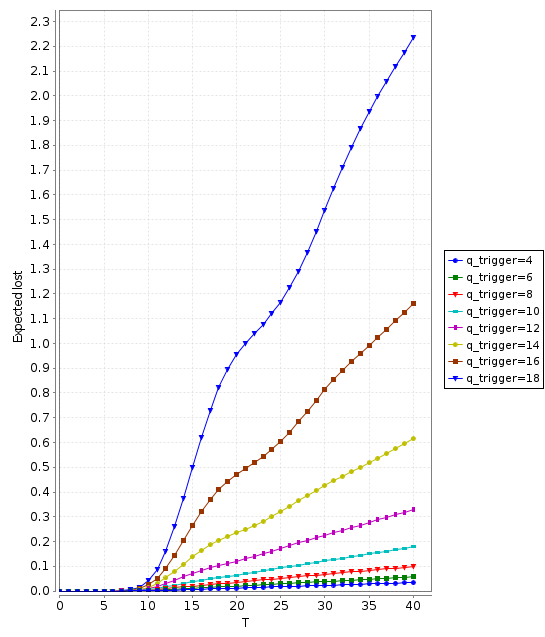
\includegraphics[width=13cm,
  height=13cm]{quantitative-project/expected-missed-requests.png}
  \caption{Expected cumulative missed number of requests}
  \label{fig:expected-cumulative-missed-requests}
\end{figure}
For greater values of $q_{trigger}$ the expected number of missed
requests increase, in fact the more time the Power Manager waits
before ``weak up'' the Service Locator, the more the queue gets bigger
and more requests could be missed.

\subsection{Transient expected cumulative power }

In this paragraph we study the last property which concern the power
consumption of the system. It isn't required to make any change to the
model, all we have to do is to build a reward structure which catch
the following specification (from \cite{QWP99}):
\begin{quote}
  Energy is used at rate 0.13, 0.95 or 2.15 for Service Provider power
  states \emph{sleep}, \emph{idle} and \emph{busy} respectively.

  Transitions between power states have a fixed energy cost: going
  from \emph{sleep} to \emph{idle} uses 7.0 units and from \emph{idle}
  to \emph{sleep} uses 0.067 units.
\end{quote}
We definite the reward structure as follow:
\begin{verbatim}
rewards "power"
	sp=0 : .13;
	sp=1 : .95;
	sp=2 : 2.15;
	[sleep2idle] true : 7;
	[idle2sleep] true : .067;
endrewards
\end{verbatim}

In \autoref{fig:expected-cumulative-power} we report the results of the
experiment the following property which uses the structure just
defined:
\begin{displaymath}
  R\{"power"\}_{=?} [ C<=T ]
\end{displaymath}
\begin{figure}[htb]
  \centering
  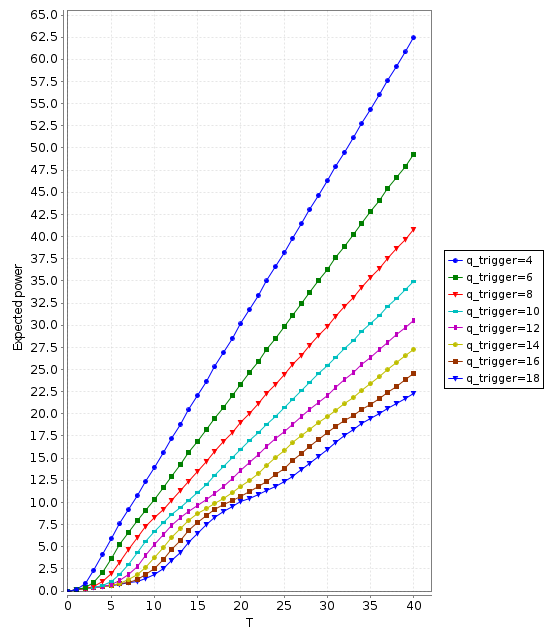
\includegraphics[width=13cm,
  height=13cm]{quantitative-project/expected-power.png}
  \caption{Expected cumulative power}
  \label{fig:expected-cumulative-power}
\end{figure}
It is not surprising to see that the power consumption for
$q_{trigger}=18$ is the lowest: when $q_{trigger} = 18$ the expected
queue size is very unstable, hence in the queue would be requests
waiting for Service Provider. In that case the Service Provider will
remain in its \emph{busy} state, limiting the number of transitions
between the other two states ($sleep \rightarrow idle$ is particular
heavy) paying twice the cost of being in \emph{idle} state.

\subsection{Third model: using \emph{stochastic policies}}

In this paragraph we'll study the last model concerning DPM
schemes. We use three components as in previous model but we introduce
little changes in the Power Manager in order to apply \emph{stochastic
  policies} on the transition $idle \rightarrow sleep$, the more
expensive transition. Specifically we build a new version of the Power
Manager module such that:
\begin{itemize}
\item insert a boolean variable which indicates if the transition has
  to be performed or not. This variable is used as a guard for the
  command which synchronize with the Service Provider to make it go to
  ``sleep'';
\item the synchronization command to ``wake up'' the Service Provider
  now happen only when the queue is full, hence we remove the freedom
  degree $q_{trigger}$ because it is useless in this new setting;
\item insert a new command that makes the Power Manager synchronize
  with the other components when the last request present in the queue
  is finally delivered. As update it use a new freedom degree
  $p_{sleep} \in [0,1]$ which represent the probability to set the new
  variable explained two points before, that is the probability for
  the transition $idle \rightarrow sleep$ to take place.
\end{itemize}

We can observe that for the minimum and maximum values of $p_{sleep}$
we have, assuming the system is neither in its initial state (where
the Service Provider is in \emph{sleep} state) nor in the first
interval time such that the queue hasn't reached the \emph{full}
state:
\begin{itemize}
\item if $p_{sleep} = 0$ then the Service Provider will never reach
  the \emph{sleep} state because the Power Manager always reset its
  internal variable that allow the $idle \rightarrow sleep$ transition;
\item if $p_{sleep} = 1$ then the Service Provider will reach the
  \emph{sleep} state every time it is possible, because the Power
  Manager always set its internal variable that allow the $idle
  \rightarrow sleep$ transition.
\end{itemize}

We've repeated the same verification of the last three properties
reported for the second model with $p_{sleep} \in {0, .2, .4, .6, .8,
  1}$. In \autoref{fig:expected-queue-size-psleep},
\autoref{fig:expected-missed-requests-with-psleep} and
\autoref{fig:expected-power-psleep} we report the plots which
corresponds to those of the previous model about the expected queue
size, the expected cumulative missed requests and the expected power
respectively.
\begin{figure}[htb]
  \centering
  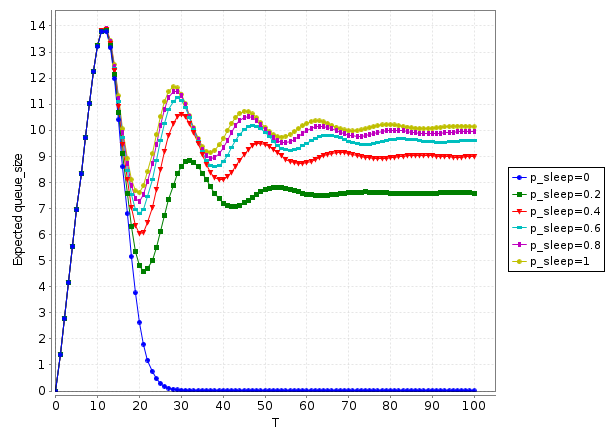
\includegraphics[width=13cm]{quantitative-project/expected-queue-size-with-psleep.png}
  \caption{Expected queue size with multiple $p_{sleep}$}
  \label{fig:expected-queue-size-psleep}
\end{figure}

\begin{figure}[htb]
  \centering
  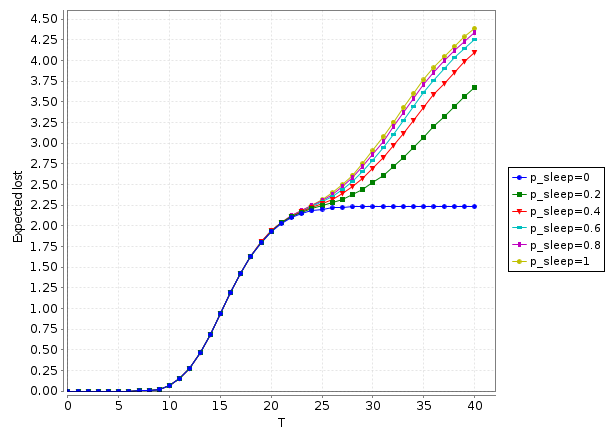
\includegraphics[width=13cm]{quantitative-project/expected-missed-requests-with-psleep.png}
  \caption{Expected missed requests with multiple $p_{sleep}$}
  \label{fig:expected-missed-requests-with-psleep}
\end{figure}
\begin{figure}[htb]
  \centering
  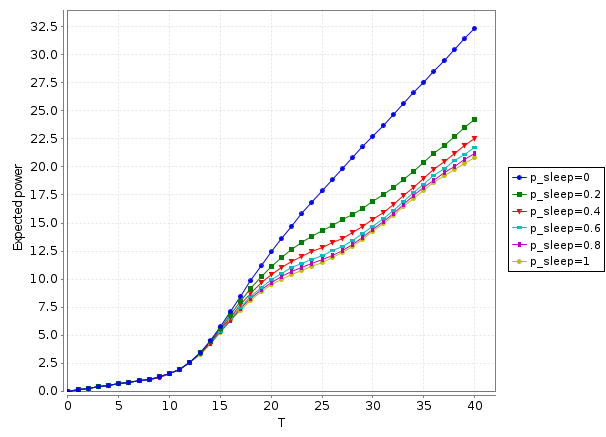
\includegraphics[width=13cm]{quantitative-project/expected-power-with-psleep.png}
  \caption{Expected power with multiple $p_{sleep}$}
  \label{fig:expected-power-psleep}
\end{figure}
We see that, for $p_{sleep} = 0$ in the long run the expected queue
size is 0 (because the Service Provider ``never sleeps''), the
expected number of missed requests stabilizes around 2.25 (while for
greater values of $p_{sleep}$ the missed requests diverge) and the
expected power is the greatest respect to greater values of
$p_{sleep}$ (being always active has its drawbacks).

Instead, for $p_{sleep} = 1$ in the long run the expected queue size
is the greatest (because the Service Provider ``sleeps as much as it
can''), the expected number of missed requests diverges and the
expected power is the lowest (being ``as lazy as possible'' produce
less power consumption).









































